\documentclass[12pt]{beamer}

% For fast compiling
%\includeonlylecture{intro}

% -- PACKAGES -- 
\usepackage{pgf}
\usepackage{pgfplots}
\usepackage{tikz}
\usetikzlibrary{patterns}
\usepackage{amsmath,amssymb,amsopn}
\usepackage[latin1]{inputenc}
\usepackage[english]{babel}
\usepackage{booktabs,colortbl}
\usepackage{subfigure}
\usepackage{import}
%\usepackage{algorithm}
\usepackage{algorithm}
%\usepackage{algorithmic}
\usepackage[noend]{algpseudocode}

\usepackage{graphicx}
\usepackage{cleveref}
\graphicspath{{./img/}}
%\newtheorem{lemma}[theorem]{Lemma}

\usepackage[normalem]{ulem}


\usepackage{biblatex}
\addbibresource{ref.bib}
\addbibresource{jcc-bib.bib}
\addbibresource{msip-bib.bib}
\addbibresource{dfo-bib.bib}



%-- Beamer setup --%

% Colors
%\definecolor{wisconsin-gold}{rgb}{0.8,0.6,0}
\definecolor{lehigh-gold}{rgb}{1,0.9,0.1}
\definecolor{wisconsin-red}{rgb}{0.6,0,0}

\definecolor{french-blue}{rgb}{0,0.1254,0.62}
\definecolor{french-red}{rgb}{0.96,0.16,0.25}

 \definecolor{myblue1}{RGB}{35,119,189}
    \definecolor{myblue2}{RGB}{95,179,238}
    \definecolor{myblue3}{RGB}{129,168,207}
    \definecolor{myblue4}{RGB}{26,89,142}


\setbeamercolor*{structure}{fg=myblue1,bg=blue}
    \setbeamercolor*{palette primary}{use=structure,fg=white,bg=structure.fg}
    \setbeamercolor*{palette secondary}{use=structure,fg=white,bg=structure.fg!75!black}
    \setbeamercolor*{palette tertiary}{use=structure,fg=white,bg=structure.fg!50!black}
    \setbeamercolor*{palette quaternary}{fg=black,bg=white}

    \setbeamercolor*{item projected}{fg=red,bg=myblue3!80}
    \setbeamercolor*{block title example}{fg=white,bg=myblue4}
    \setbeamercolor*{frametitle}{fg=myblue4,bg=white}

    \setbeamertemplate{blocks}[rounded][shadow=true]

    \makeatletter
    \pgfdeclarehorizontalshading[frametitle.bg,frametitle right.bg]{beamer@frametitleshade}{\paperheight}{%
      color(0pt)=(myblue2);
      color(\paperwidth)=(white)}

    \defbeamertemplate*{footline}{mysplit theme}
    {%
      \leavevmode%
      \hbox{\begin{beamercolorbox}[wd=.5\paperwidth,ht=2.5ex,dp=1.125ex,leftskip=.3cm plus1fill,rightskip=.3cm]{author in head/foot}%
        \usebeamerfont{author in head/foot}\insertshortauthor
      \end{beamercolorbox}%
      \begin{beamercolorbox}[wd=.5\paperwidth,ht=2.5ex,dp=1.125ex,leftskip=.3cm,rightskip=.3cm plus1fil]{title in head/foot}%
        \usebeamerfont{title in head/foot}\insertshorttitle\hfill
        \insertframenumber/\inserttotalframenumber\hspace*{0.5em}
      \end{beamercolorbox}}%
      \vskip0pt%
    }
    \makeatother




\tikzset{
        hatch distance/.store in=\hatchdistance,
        hatch distance=10pt,
        hatch thickness/.store in=\hatchthickness,
        hatch thickness=2pt
    }

\makeatletter
    \pgfdeclarepatternformonly[\hatchdistance,\hatchthickness]{flexible hatch}
    {\pgfqpoint{0pt}{0pt}}
    {\pgfqpoint{\hatchdistance}{\hatchdistance}}
    {\pgfpoint{\hatchdistance-1pt}{\hatchdistance-1pt}}%
    {
        \pgfsetcolor{\tikz@pattern@color}
        \pgfsetlinewidth{\hatchthickness}
        \pgfpathmoveto{\pgfqpoint{0pt}{0pt}}
        \pgfpathlineto{\pgfqpoint{\hatchdistance}{\hatchdistance}}
        \pgfusepath{stroke}
    }


\makeatletter
    \pgfdeclarepatternformonly[\hatchdistance,\hatchthickness]{flexible hatch2}
    {\pgfqpoint{0pt}{0pt}}
    {\pgfqpoint{\hatchdistance}{\hatchdistance}}
    {\pgfpoint{\hatchdistance-1pt}{\hatchdistance-1pt}}%
    {
        \pgfsetcolor{orange}
        \pgfsetlinewidth{\hatchthickness}
        \pgfpathmoveto{\pgfqpoint{0pt}{0pt}}
        \pgfpathlineto{\pgfqpoint{\hatchdistance}{\hatchdistance}}
        \pgfusepath{stroke}
    }




% -- Images you want to use more than once --

%\pgfdeclareimage[width=1cm]{wisconsin-logo}{images/wcrest} 
%\logo{\pgfuseimage{wisconsin-logo}}


%\pgfdeclareimage[width=0.1\textwidth]{flag-small}{images/Flag_of_France}


% -- Jeff's MACROS -- %

\newcommand{\picframetitle}[2]{
    \vskip0.25em%
    \begin{centering}
      \begin{minipage}[c]{0.7\linewidth}
	\Large \alert{#1}
      \end{minipage} \hfill
      \begin{minipage}[c]{0.22\linewidth}
	\pgfimage[height=0.5in]{#2}
      \end{minipage}
      \par
    \end{centering}
}

\newcommand{\medpicframetitle}[2]{
    \vskip0.25em%
    \begin{centering}
      \begin{minipage}[c]{0.7\linewidth}
	\Large \alert{#1}
      \end{minipage} \hfill
      \begin{minipage}[c]{0.22\linewidth}
	\pgfimage[height=0.75in]{#2}
      \end{minipage}
      \par
    \end{centering}
}

\newcommand{\bigpicframetitle}[2]{
    \vskip0.25em%
    \begin{centering}
      \begin{minipage}[c]{0.7\linewidth}
	\Large \alert{#1}
      \end{minipage} \hfill
      \begin{minipage}[c]{0.22\linewidth}
	\pgfimage[height=1in]{#2}
      \end{minipage}
      \par
    \end{centering}
}

\newcommand{\bigpicframetitletwo}[2]{
    \vskip0.25em%
      \begin{minipage}[c]{0.6\linewidth}
	\Large \alert{#1}
      \end{minipage} \hfill
      \begin{minipage}[c]{0.32\linewidth}
	\hfill \pgfimage[height=0.8in]{#2}
      \end{minipage}
      \par
}

\newcommand{\bigpicframetitlethree}[2]{
    \vskip0.25em%
      \begin{minipage}[c]{0.6\linewidth}
	\Large \alert{#1}
      \end{minipage} \hfill
      \begin{minipage}[c]{0.32\linewidth}
	\hfill \pgfimage[height=0.8in]{#2}
      \end{minipage}
      \par
}

\newcommand{\bi}{\begin{itemize}}
\newcommand{\ei}{\end{itemize}}
\newcommand{\BI}{\begin{itemize}}
\newcommand{\EI}{\end{itemize}}
\newcommand{\BEN}{\begin{enumerate}}
\newcommand{\EEN}{\end{enumerate}}

\newcommand{\BBR}[1]{\begin{beamerboxesrounded}[shadow=true,width=0.96\textwidth]{\color{lehigh-gold}#1}}
\newcommand{\EBR}{\end{beamerboxesrounded}}

\newcommand{\BCS}{\begin{columns}}
\newcommand{\BC}[1]{\begin{column}{#1\linewidth}}
\newcommand{\EC}{\end{column}}
\newcommand{\ECS}{\end{columns}}

\newcommand{\MSS}{\medskip\alert{\hrule}\medskip}
\newcommand{\BSS}{\bigskip\alert{\hrule}\bigskip}
\newcommand{\st}{\; | \;}

\newcommand{\noprint}[1]{}
\newcommand{\exclude}[1]{}
\newcommand{\cB}{{\cal B}}
\newcommand{\cC}{{\cal C}}
\newcommand{\cD}{{\cal D}}
\newcommand{\cE}{{\cal E}}
\newcommand{\cF}{{\cal F}}
\newcommand{\cG}{{\cal G}}
\newcommand{\cI}{{\cal I}}
\newcommand{\cK}{{\cal K}}
\newcommand{\cL}{{\cal L}}
\newcommand{\cN}{{\cal N}}
\newcommand{\cO}{{\cal O}}
\newcommand{\cP}{{\cal P}}
\newcommand{\cQ}{{\cal Q}}
\newcommand{\cR}{{\cal R}}
\newcommand{\cS}{{\cal S}}
\newcommand{\cT}{{\cal T}}
\newcommand{\cU}{{\cal U}}
\newcommand{\cX}{{\cal X}}
\newcommand{\cV}{{\cal V}}
\newcommand{\cZ}{{\cal Z}}

\newcommand{\magE}{\left| \mathcal{E} \right|}

\newcommand{\defeq}{\stackrel{\rm def}{=}}
\newcommand{\Expect}{\mathbb{E}}

\newcommand{\orb}{\operatorname{orb}}


\newcommand{\ry}{\pmb{y}}
\newcommand{\rye}{\pmb{y_e}}

\makeatletter
\def\BState{\State\hskip-\ALG@thistlm}
\makeatother


\defbeamertemplate*{title page}{customized}[1][]
{
  \usebeamerfont{title}\inserttitle\par
  \usebeamerfont{subtitle}\usebeamercolor[fg]{subtitle}\insertsubtitle\par
  \bigskip
  \bigskip
  \bigskip
  \begin{tabular}{ c l}
    \begin{tabular}{c}
  \usebeamercolor[fg]{titlegraphic}\inserttitlegraphic \\

  \usebeamerfont{institute}\insertinstitute
    \end{tabular} 
    & 
    \begin{tabular}{l}
    \usebeamerfont{author}\insertauthor \\
    \usebeamerfont{date}\insertdate
    \end{tabular} 
\end{tabular}
}

\newcommand{\mypathbase}{/home/eric/work/present/ases-present}
\newcommand{\mypathdata}{\mypathbase/data}
\newcommand{\mypathjcc}{\mypathbase/jcc}
\newcommand{\mypathjccdata}{\mypathbase/jcc/data}
\newcommand{\mypathdfo}{\mypathbase/dfo}
\newcommand{\mypathimg}{\mypathbase/img}
\newcommand{\bc}[1]{}
\newcommand{\bE}{\mathbb{E}}
\newcommand{\bD}{\mathbb{D}}
\newcommand{\E}[2]{\mathbb{E}_{#1} \left[ #2 \right]}
\newcommand{\bP}[2]{\mathbb{P}_{#1} \left[ #2 \right]}
\newcommand{\dpO}{d\mathbb{P}_\Omega}
\newcommand{\feb}{f_e\left(\beta\right)}
\newcommand{\fenb}{f_{en}\left(\beta\right)}
\newcommand{\fehb}{f_e\left(\hat{\beta}\right)}
\newcommand{\pfeb}{\frac{\partial}{\partial \beta_j}\feb}
\newcommand{\pfenb}{\frac{\partial f_{en}\left(\beta \right)}{\partial \beta_j}}
\newcommand{\pfehb}{\frac{\partial f_e\left(\hat{\beta} \right)}{\partial \beta_j}}
\newcommand{\hye}{\hat{y}_e}
\newcommand{\hse}{\hat{s}_e}
\newcommand{\pe}{\pi_e}
\newcommand{\pn}{\pi_n}
\newcommand{\psen}{\psi_{en}}
\newcommand{\rand}{\boldsymbol{\delta}}
\newcommand{\ri}{\pmb{\delta^m}}
\newcommand{\rf}{\pmb{\delta^y}}
\newcommand{\rx}{\pmb{x}}
\newcommand{\rX}{\pmb{X}}
\newcommand{\rD}{\pmb{\Delta}}
\newcommand{\rdm}{\pmb{\delta^m}}
\newcommand{\rdmk}{\pmb{\delta^m_k}}
\newcommand{\rdy}{\pmb{\delta^y}}
\newcommand{\hry}{\pmb{y}}
\newcommand{\hy}{y}
\newcommand{\rz}{\pmb{z}}
\newcommand{\sD}{\sigma_\Delta^2}
\newcommand{\se}{\sigma_{e_1}^2}
\newcommand{\seone}{\sigma_{e_1}^2}
\newcommand{\setwo}{\sigma_{e_2}^2}
\newcommand{\sn}{\sigma_{e_2}^2}
\newcommand{\sen}{\sigma_{e_1 e_2}^2}
\newcommand{\see}{\sigma_{e_1 e_1}^2}
\newcommand{\snn}{\sigma_{e_2 e_2}^2}
\newcommand{\seealone}{\sigma_{e_1 e_2}^2}
\newcommand{\sko}{\sum_{k_1 \in \cM}}
\newcommand{\skt}{\sum_{k_2 \in \cM}}
\newcommand{\sigot}{\Sigma_{k_1,k_2}}
\newcommand{\irzp}{\E{\Omega}{g(\hry_e)}}
%\newcommand{\rw}{{w(\omega)}} %\newcommand{\rx}{{x(\omega)}} %\newcommand{\ry}{{y(\omega)}}
\newcommand{\Ery}{\E{\Omega}{\ry}}
\newcommand{\Erx}{\E{\Omega}{\rx}}
\newcommand{\Erdm}{\E{\Omega}{\rdm}}
\newcommand{\ErD}{\E{\Omega}{\rD}}
\newcommand{\tB}{\tilde{B}}
\newcommand{\tx}{\tilde{x}}
\newcommand{\ttheta}{\tilde{\theta}}

\title[Reliability and Renewable Generation]{Line Failure Risk from Congestion}
\subtitle{Incorporating Uncertainty in Renewable Generation}
\author{Eric Anderson}
\institute{Anderson Optimization }

\date{Presentation for PIMS at UBC \\
  Wednesday, May 22nd, 2019}
\titlegraphic{
\includegraphics[scale=0.15]{logo}}
\begin{document}

\begin{frame}
\titlepage
\end{frame}



\begin{frame}{My Background}

\bi
\item Ph.D. in Industrial Engineering from UW-Madison
\item Focus on optimization models for power systems
\bi
\item Cascading power failures
\item Dispatch models incorporating renewable generation
\item Themes of large scale computation and uncertainty
\ei
\item This talk is based on my thesis research with 
\bi
\item Jeff Linderoth, Jim Luedtke, and Bernard Lesieutre
\ei
\ei

\end{frame}
\begin{frame}{Anderson Optimization}

\bi
\item Startup for energy analysis software
\item Primary clients are renewable developers
\bi
\item Mostly solar, some wind, some battery analysis
\ei
\ei
\pause
\bi
\item Web platform for energy analysis
\bi
\item Prospecting for development sites
\item Early stage economic and feasibility analyis
\item Production cost modeling
\ei
\ei

\end{frame}
\begin{frame}{Why I'm Here}

\bi
\item Interested in both clean energy and math!
\item Potential colloboration in the future
\item Potential clients 
\item Great location!
\ei 

\end{frame}

\subsubsection{Outline}
\begin{frame}{Outline}

\tableofcontents[subsubsectionstyle=hide]  

\end{frame}

\section{Overview}

\subsection{Context}
\begin{frame}{Context}
\bi
\item Climate change is ongoing, want to reduce emissions
\item Reduce through increasing renewables
\ei

\pause
\centering
\vspace{.2in}
\alert{Emmissions of Electricity Generation}
\vspace{.2in}
\begin{columns}
\begin{column}{0.425\textwidth}
\centering
Canada
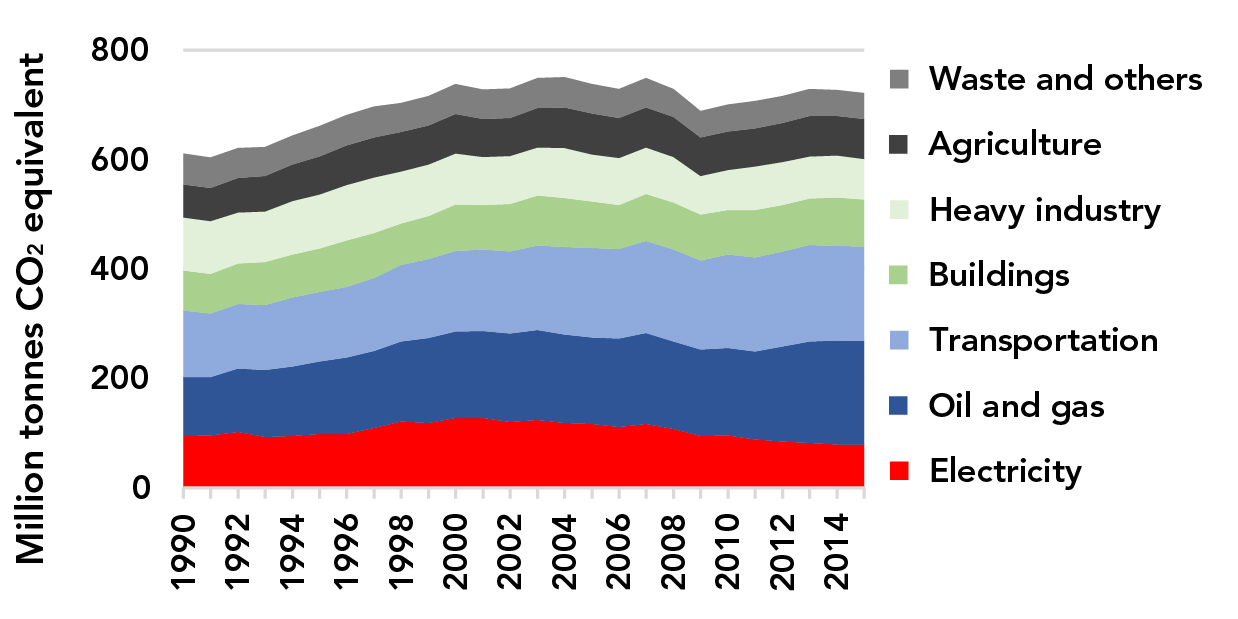
\includegraphics[height=1.15in]{ghg_emissions}
\end{column}
\begin{column}{0.425\textwidth}
\centering
Worldwide
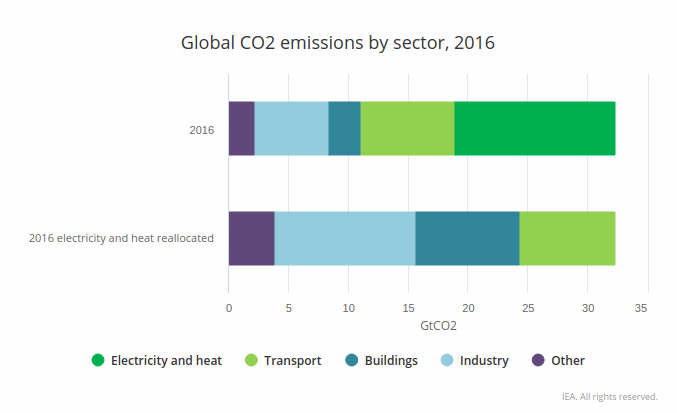
\includegraphics[height=1.15in]{ghg_emissions_worldwide}
\end{column}
\end{columns}
\end{frame}

\subsection{Power Systems Analysis}
\begin{frame}{Challenges}


\BBR{Bulk Power Systems (BPS)}
\bi
\item Composed of generation and high voltage transmission equipement.  
\item Goal to serve load with least cost electricity while maintaining reliability.
\ei
\EBR
\pause
\vspace{.3in}
\alert{Challenges}
\bi
\item Renewables [often] connect with bulk power system (BPS)
\item BPS must maintain system reliability
\item Renewables uncertain and not controllable
\ei
\end{frame}

\begin{frame}{Bulk Power Systems}

\only<1>{US split into 3 interconnected grids}
\only<2>{\sout{US split into 3 interconnected grids}}

\only<2>{\alert{North America split into 4 interconnected grids}}
\bi
\item Generators rotating synchronously with grid
\item Connection to every load
\ei



\end{frame}

\begin{frame}{North America Interconnections}
\centering
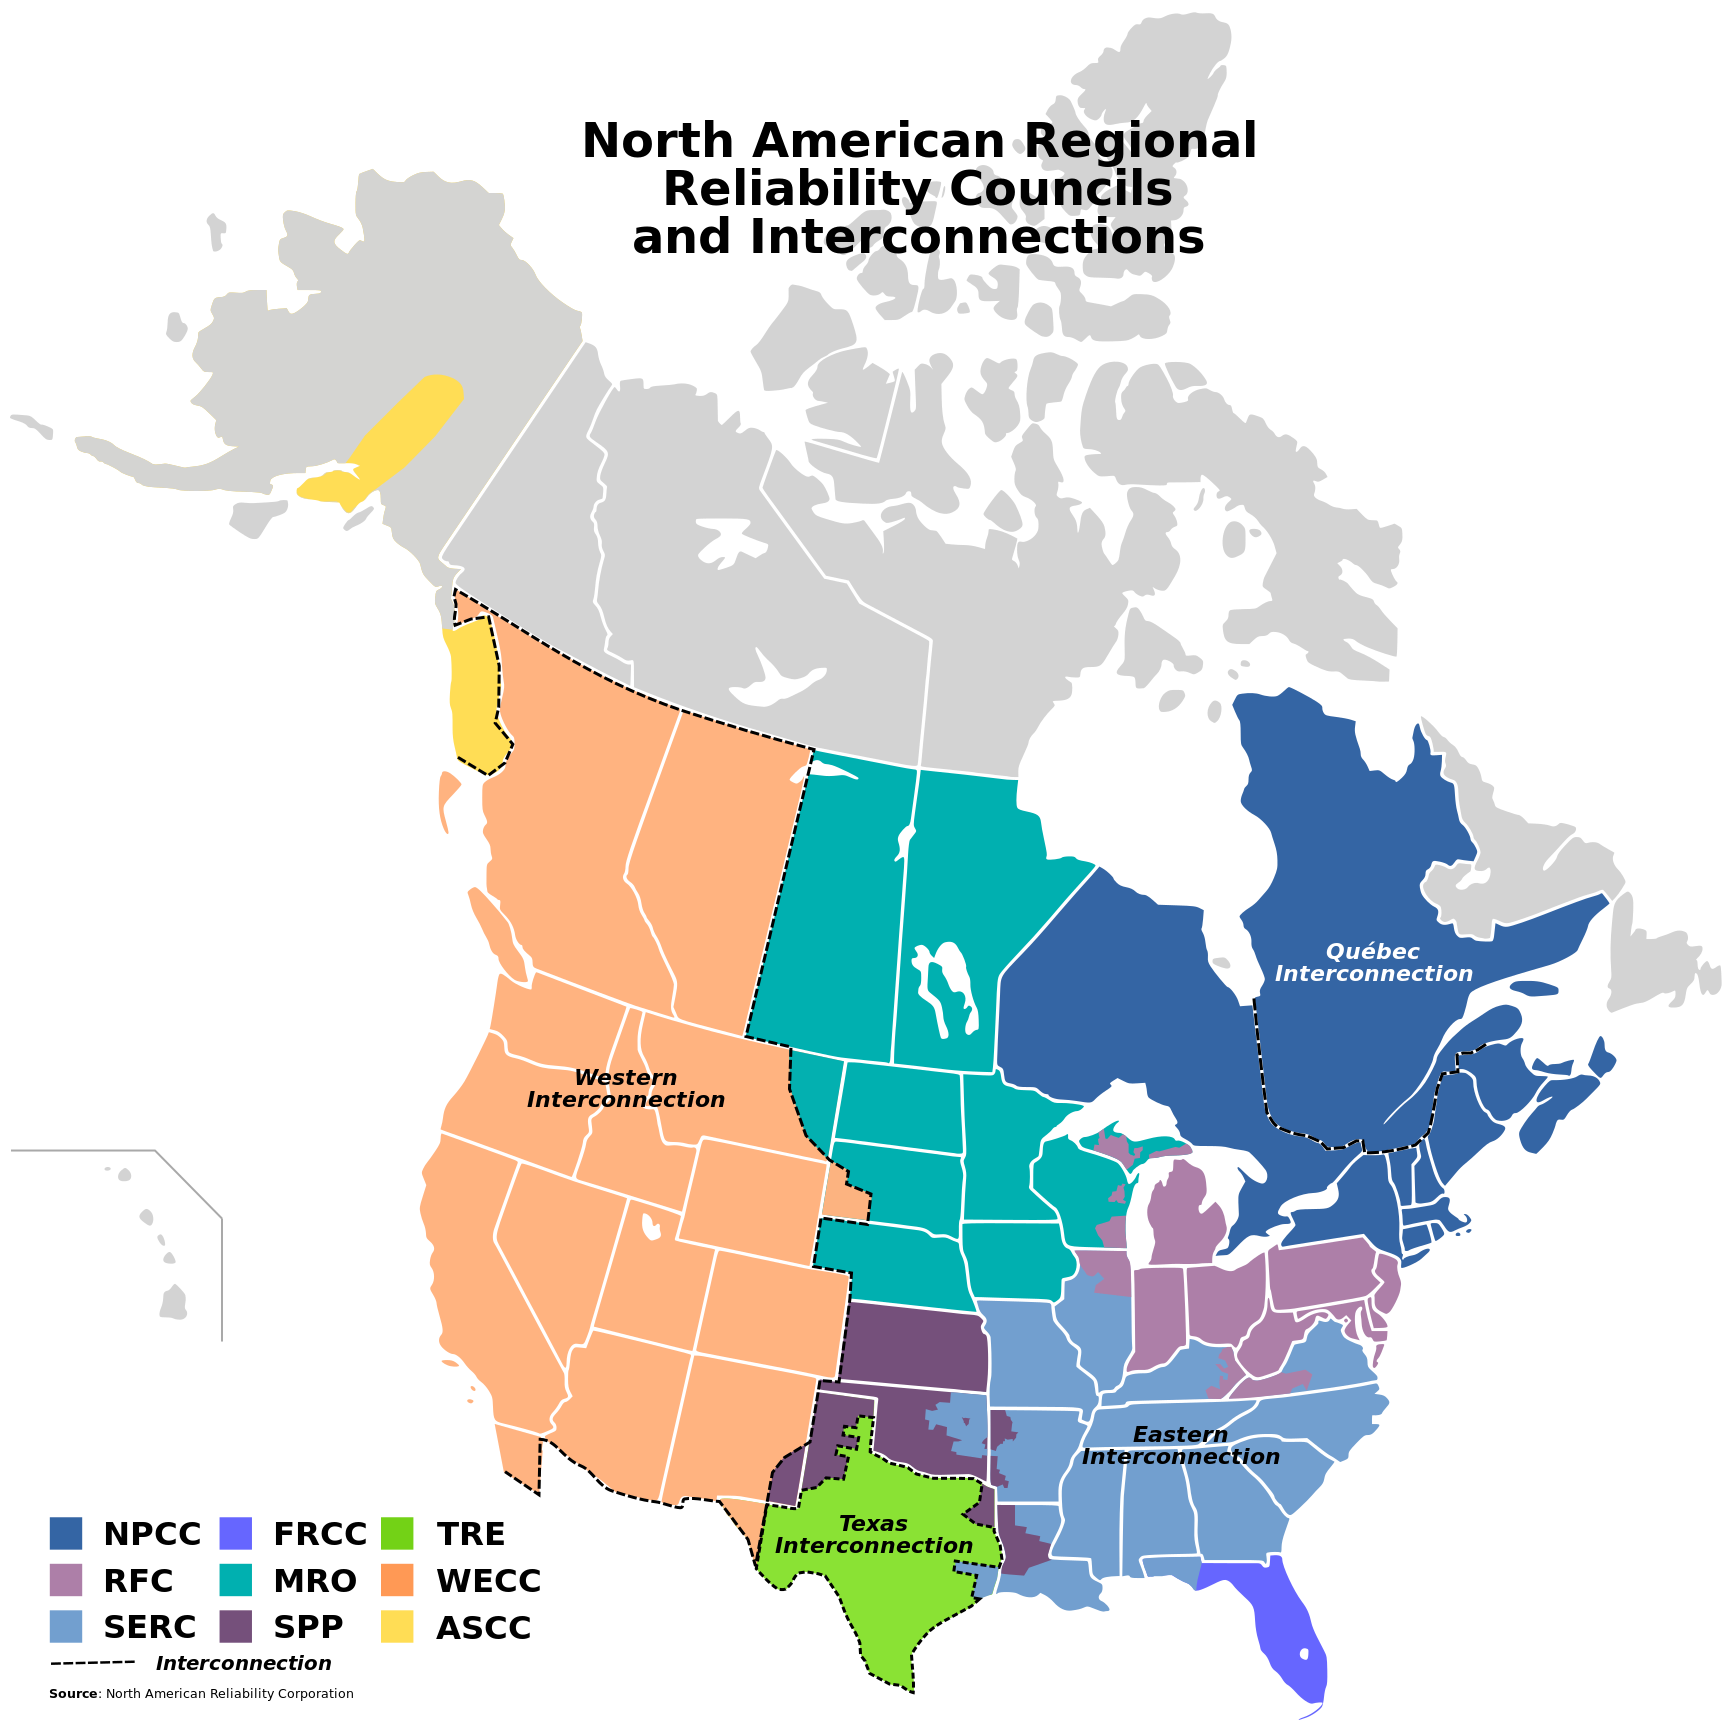
\includegraphics[height=3in]{interconnect.png}
\end{frame}

\begin{frame}{Bulk Power Systems}


Complex system requiring continuous supply demand balance

\bi
\item Transient stability, automatic generator control
\item Ancillary services market
\item \only<1>{ 5 minute real time market} \only<2>{\textcolor{red}{ 5 minute real time market}} 
\item 1-6 hour inter region market 
\item 24 hour day ahead market
\item Long term capacity markets
\ei
\end{frame}

\begin{frame}{Optimization in Power System}

\bi
\item Operational/Markets
	\bi
	\item Real time market / economic dispatch \only<2>{- \textcolor{red}{LP}}
	\item Day ahead market / unit commitment \only<2>{- \textcolor{red}{MIP}}
	\ei
\item Planning
	\bi
	\item Production cost model
		\only<2>{ \textcolor{red}{simulation - MIP}}
	\item Capacity expansion 
		\only<2>{\textcolor{red}{MIP / DFO}}
	\ei
\item Reliability
	\bi
	\item Power flow / optimal power flow \only<2>{- \textcolor{red}{NLP}}
	\item Dynamics / transient stability \only<2>{\textcolor{red}{simulation - NLP}}
	\ei
\ei


\only<2>{
\bi
	\item \textcolor{red}{LP} = Linear Program
	\item \textcolor{red}{MIP} = Mixed Integer Program
	\item \textcolor{red}{NLP} = Nonlinear Program
	\item \textcolor{red}{DFO} = Derivative Free Optimization
\ei}

\end{frame}

\begin{frame}{Power Flow}
Laws of physics, can't control branch flow

\alert{Control net injects}
\bi
\item Generators
\bi 
\item Ramping characterstics, limits
\ei
\item Demand Response
\item Storage (hydro, battery)
\ei

\pause

AC power flow - balanced 3 phase power system model 
\bi
\item Nonlinear, nonconvex equations
\item Difficult to solve
\item \alert{We use DC approximation (linear)}
\ei

%3 ways to solve
%\bi
%\item Local methods (i.e. Newton method, no optimality guarantees)
%\item Convex Relaxations (i.e. SDP [Lavaei and Low], Quadratic [Hijazi]) %put in footnote
%\bi
%\item Ability to distinguish numerical problems from systemic infeasibility
%\ei
%\item Approximations (i.e. DC power flow, linear approximation)
%\bi
%\item Reduction in computational complexity at cost to accuracy
%\item Extensions to capture voltage information and transmission losses
%\ei
%\ei
\end{frame}

\begin{frame}{ERCOT Snapshot}

\vspace{-4cm}
\hspace{-2cm}
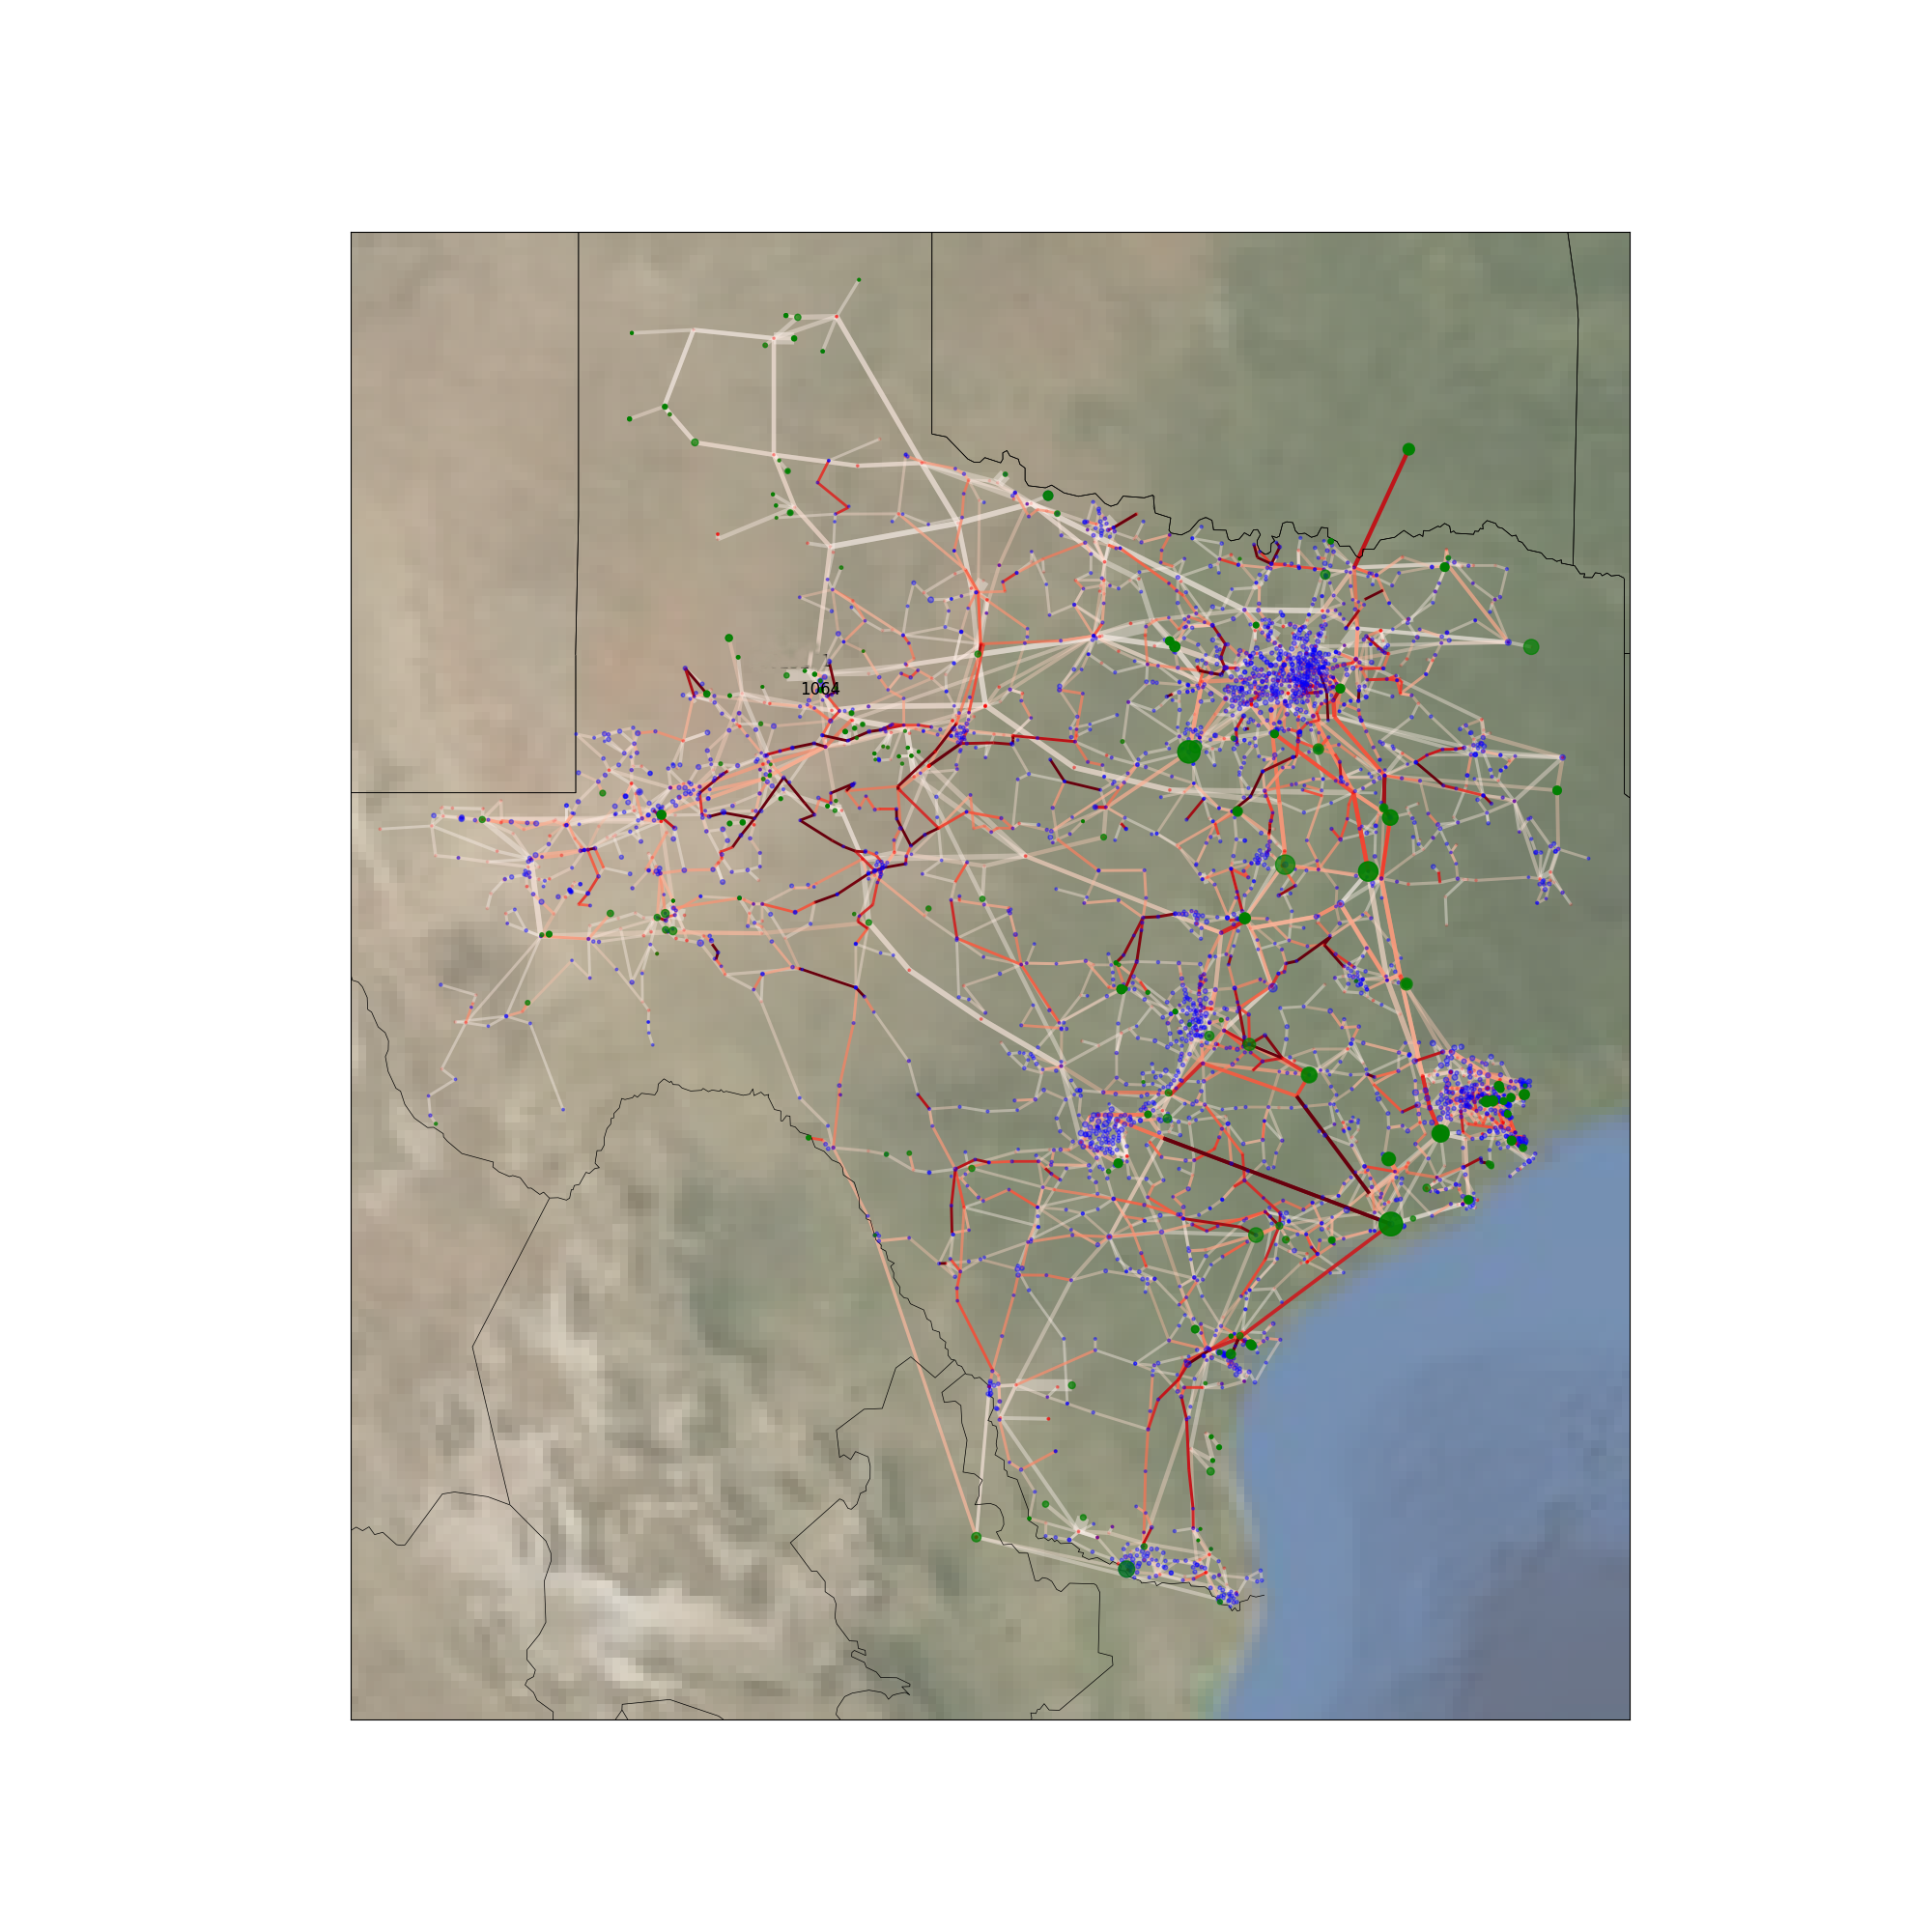
\includegraphics[height=6in,width=5in,trim={5cm 5cm 5cm 5cm},clip]{ercot_example.png}
\end{frame}

\subsection{Uncertainty}
\begin{frame}{Modern Complexity for Power Systems}

\alert{Uncertainty}

Asking more of our transmission grid, robust to uncertainty

\bi
\item Wind
\item Solar
\item Demand Response
\item Energy Storage
\item Electric Vehicles
\ei
\end{frame}

\bc{
\begin{frame}{Renewable Generation, Geographically Correlated}
\begin{center}
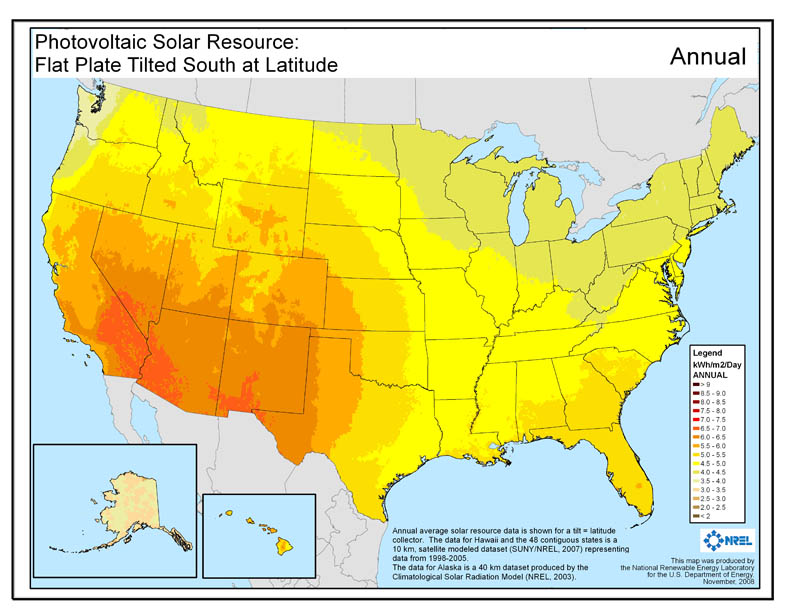
\includegraphics[height=1.4in]{solar-map} \hfill %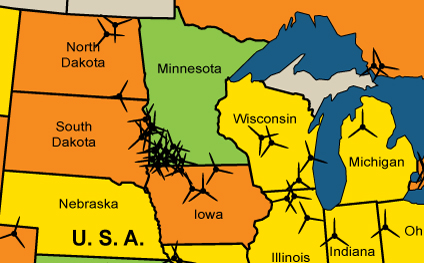
\includegraphics[height=1.4in]{windmap}
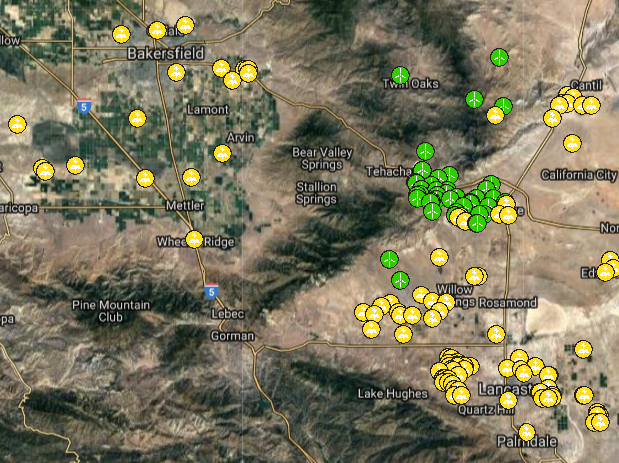
\includegraphics[height=1.4in]{renewables-correlated}
\end{center}
\end{frame}
}

\subsection{Reliability Problems}
\begin{frame}{Reliability Problems}
\alert{Power Interruptions}
\bi
\item \$79 billion economic loss (2001) 
\bi
\item \$247 billion electricity sales
\ei 
\item Hidden from system, distributed throughout economy
\item New technologies: renewables, EVs, etc. stressful on system
\ei
\pause
\alert{Cascading power failures}
\bi
\item Rare, but costly
\item Equillibrium balancing economics and reliability
\item Northeast blackout 2003
\bi
\item \$6 billion economic loss
\item Loss of life
\ei
\ei
\end{frame}

\section{Incorporating Uncertainty}
\frame{\tableofcontents[currentsection,subsubsectionstyle=hide]}

\subsection{Uncertain Injects}
\bc{\begin{frame}{Uncertain Injects}
\alert{Uncertainty in Injects to Power System}
\bi
\item Subset of nodes have uncertain injections
\bi
\item Solar, wind
\item Demand (relatively certain, however EVs could represent change)
\ei
\pause
\item Subset of assets respond to uncertainty (slack distribution)
\bi
\item Rotational inertia, peaker plants and regulation
\item Energy storage, enhanced power controls
\ei
\ei
\end{frame}
}

\begin{frame}{Uncertainty is Multivariate Normal}
\alert{Assumption}

Uncertainty in net injections are Multivariate Normal
\bi
\item \textit{Uncertainty in errors from forecast}
\item Known or can be empirically estimated
\item Potentially correlated
\ei
\begin{center}
% 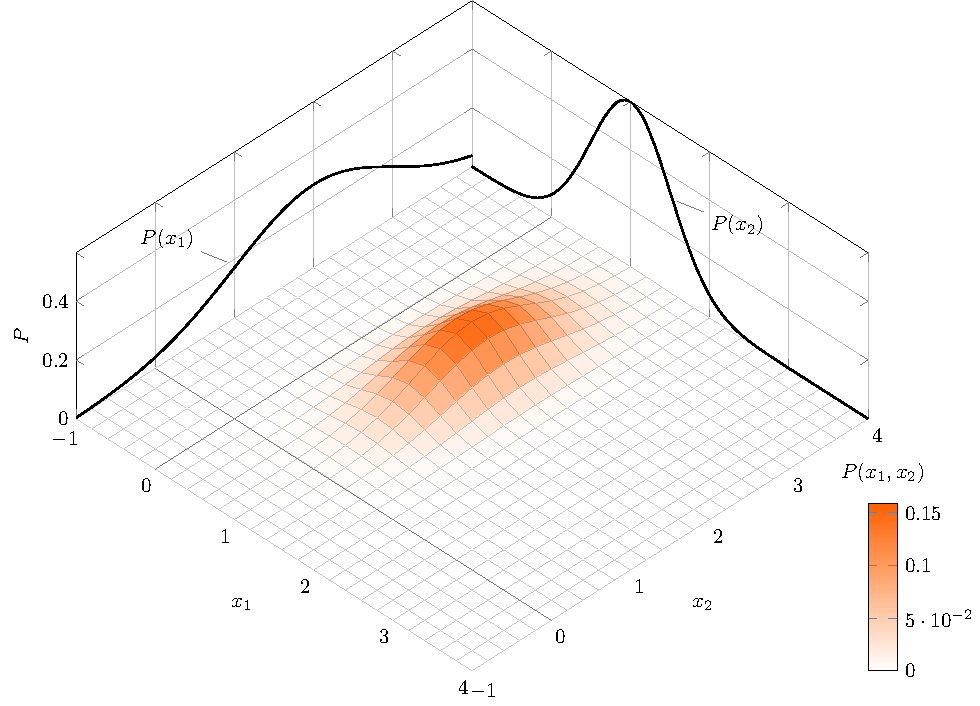
\includegraphics[scale=.325]{multivariate} 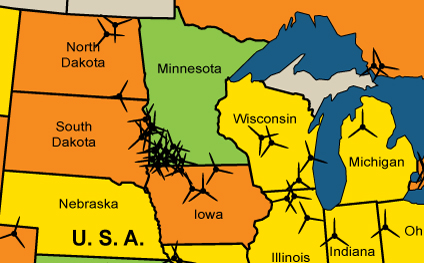
\includegraphics[scale=.35]{windmap}
\begin{figure}
   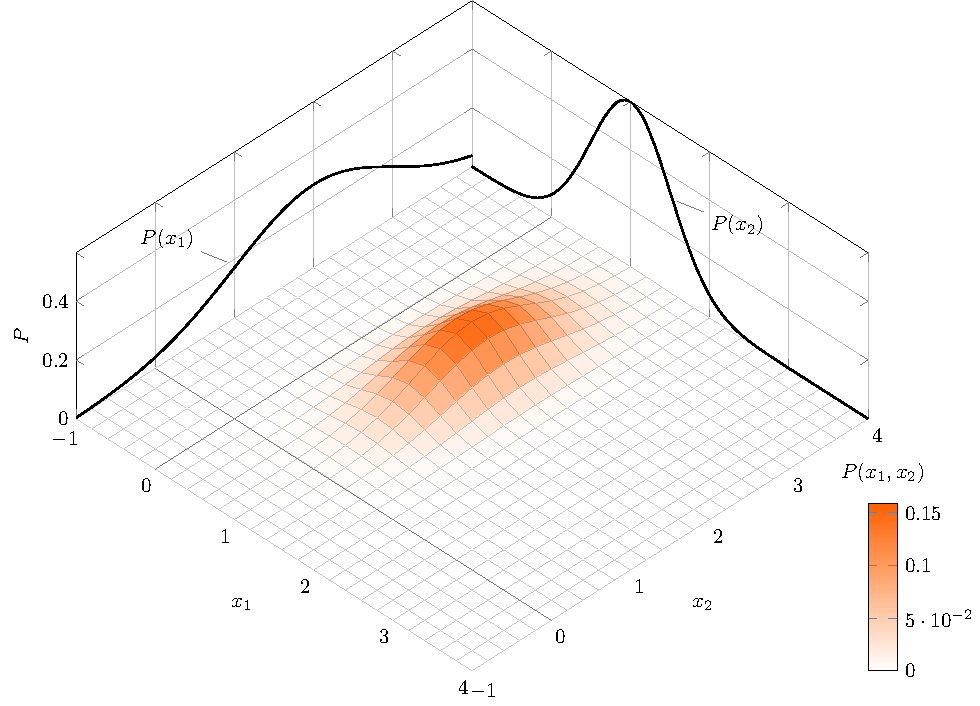
\includegraphics[width=0.475\textwidth]{multivariate}
   \hfill
   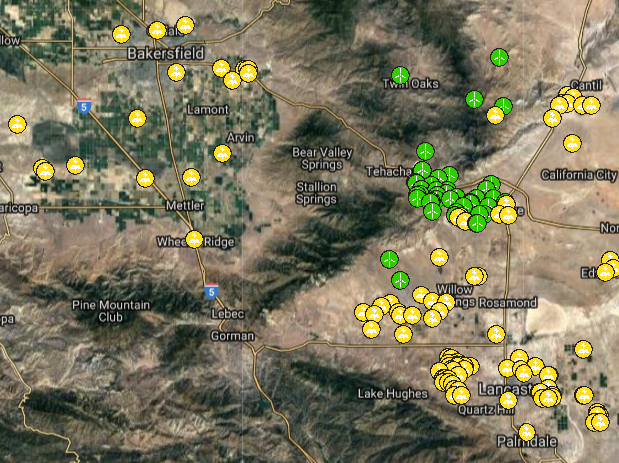
\includegraphics[width=0.475\textwidth]{renewables-correlated}
\end{figure}
\end{center}
%Error from short term forecast for windfarms is normally distributed

\end{frame}



\subsection{Issues with Deterministic Analysis}
\begin{frame}{Issues with Deterministic Analysis}
Normal distributed injects 
\pause 
$\rightarrow $
\textbf{Normal branch flows}\footnotemark
\vspace{20px}
\footnotetext[1]{In a stable system}
\pause
\alert{Problem!}
\bi
\item Branch constraints violated half the time when at its limit
\ei
\end{frame}

\begin{frame}{Normal Branch Flow}
\begin{center}
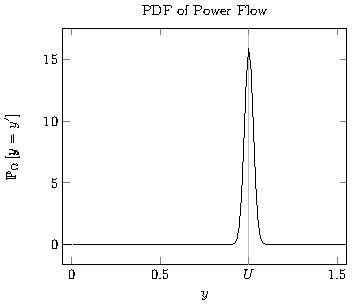
\includegraphics[scale=1.1]{\mypathjcc/fig-ccflow}
\end{center}
PDF for Branch flow with mean (forecast) at nominal capacity
\end{frame}


\begin{frame}{Normal Branch Flow}
\begin{center}
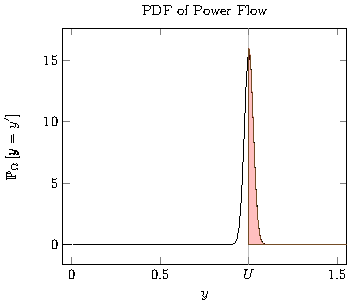
\includegraphics[scale=1.1]{\mypathjcc/fig-ccflowred}
\end{center}

\alert{Need to probabilistically enforce constraints}

\end{frame}


\subsection{Chance Constraints}
\begin{frame}{Chance Constraints}

\begin{center}
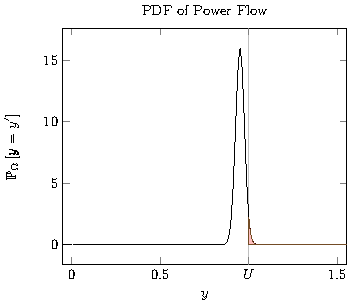
\includegraphics[scale=1.1]{\mypathjcc/fig-ccflowred-95}
\end{center}


\end{frame}

\subsection{System Risk}
\begin{frame}{Current Models}
Determinsitic has fixed line thresholds
\bi
\item Line is completely okay
\item or system is infeasible
\ei
\pause
Chance Constraints
\bi
\item Enforce line threshold probalistically
\ei
\pause

\alert{Line thresholds are soft constraints in real life}
\pause
\bi
\item Multiple line ratings (i.e. short term emergency rating)
\item Hard limit typically relay tripping
\ei
\end{frame}

\begin{frame}{Line Limits}
Limited by
\bi
\item Sagging due to current flow and line heating
\item \alert<2>{Worst case environmental conditions (seasonally)}
\item An acceptable probability of line failure
\item Enforce N-1 Reliability Constraint
\ei
\bigskip
\pause
\textbf{Dynamic line limits}
\bi
\item Real time limits based on current environmental conditions
\ei

\end{frame}

\begin{frame}{System Risk}

System risk related to line loadings (severity measure) \footnotemark
%\footfullcite{wang_2013}
\footnotetext[2]{Qin Wang and McCalley, J.D. and Tongxin Zheng and Litvinov, E.}
\pause


\vspace{10pt}
Intuition
\bi
\item Grid relatively stressed when more lines are near their limit
\ei
%Want risk measure to compare risk of line loadings
%\vspace{10pt}
\end{frame}
\begin{frame}{Line Failure Model}

Model for line failure risk

\begin{center}
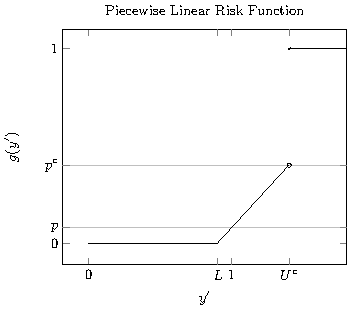
\includegraphics[scale=0.7]{\mypathjcc/fig-failuredensity}
\end{center}
\pause

Individual lines contribute to system risk
\bi
\item Balance economic object with system risk
\item Cost-risk frontier
\ei
%\vspace{50pt}
%This is the product of the probability that each line does not fail
%\begin{equation*}  
%h(y) = \prod_{e \in \cE} \left( 1 - g(y_e) \right)
%\end{equation*}  
%\bi
%\item Implies hard line constraint, line risk=system risk
%\ei
%In the static case
%\bi
%\item Perform log transform to get exact solution
%\ei

\end{frame}



% \begin{frame}{Line Risk Function}
% Risk function takes the normalized flow returns line risk 
% \begin{equation*}
%  g(\hy_e) = \bP{\Xi}{\text{Line }e\text{ fails} | \hy_e} 
% \end{equation*}
% \pause
% Piece-wise linear function choosen
% \bi
% \item Below $L$, there is no risk associated with loading
% \item After $L$, the risk increases linearly with loading
% \item At critical capacity $U^c$, line fails with certainty
% \ei
% \pause
% \begin{equation*}
% g(\hy_e) = \left\{ \begin{array}{l l}
%   0 & \hy_e \leq L \\
%   a + b \hy_e & L \leq \hy_e < U^c \\
%   1 & U^c \leq \hy_e 
% \end{array}
% \right.
% \end{equation*}
% \end{frame}

%\begin{frame}{Gaussian Branch Flow}
%\begin{center}
%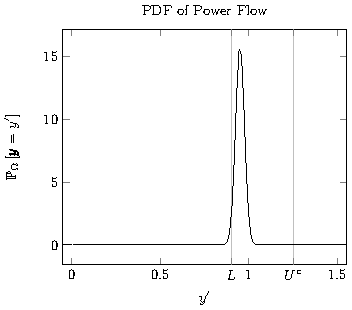
\includegraphics[scale=1.2]{\mypathjcc/fig-pdfflow}
%\end{center}
%\end{frame}






\section{Conclusion}
\begin{frame}{Solution Exploration Demo}
\url{http://eja4.info/pow-explore.html}
\bi
\item Toggle in bottom left to change dispatch model
\ei
\begin{center}
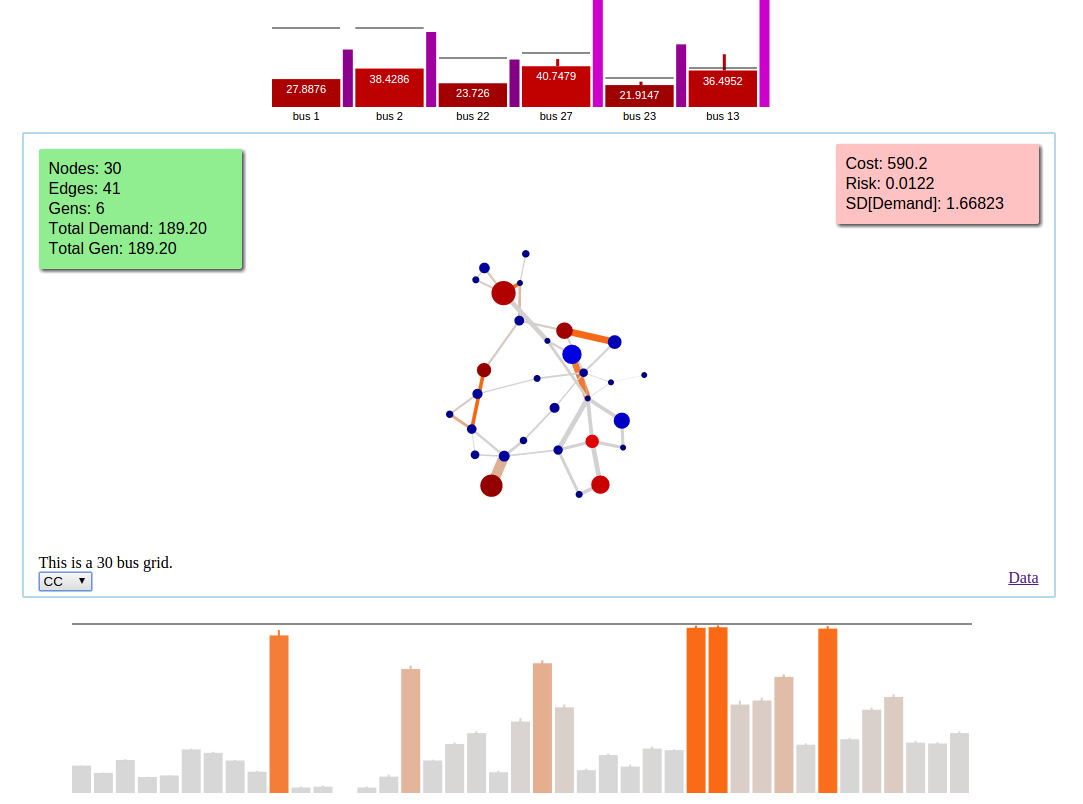
\includegraphics[scale=.22]{explore}
\end{center}
\end{frame}

\begin{frame}{Conclusion}
\bi
\item Need improved analysis for uncertainty in renewable generation
\item Correlation in renewable generation is important
\item Line failure risk vs system risk
\ei

\BBR{Thanks!}
Hope you enjoyed!

Questions?
\EBR
\end{frame}



\end{document}


